\section{Experimental Results \& Benchmarking}
\label{sec:results_benchmarking}

\subsection*{Comprehensive Benchmarking Performance Metrics}

Table~\ref{tab:comprehensive_benchmark} summarizes and benchmarks the core performance metrics across both model tiers: the Static Snapshot (evaluated at nominal coordinates $\mathbf{q}_U^{(0)} = (0.5, 0.4)$) and the Dynamic Mission Horizon ($N = 10$ time slots). Baseline references are explicitly delineated to accurately reflect performance improvement ratios.

\begin{table}[htbp]
\centering
\caption{Comprehensive Benchmarking Performance Metrics}
\label{tab:comprehensive_benchmark}
\resizebox{\textwidth}{!}{%
\begin{tabular}{|l|c|c|c|c|}
\hline
\textbf{Evaluation Metric} & \makecell{\textbf{Static Snapshot:}\\\textbf{Static AO}} & \makecell{\textbf{Dynamic Mission:}\\\textbf{Before Optimization}} & \makecell{\textbf{Dynamic Mission:}\\\textbf{Dynamic AO ($N=10$)}} & \makecell{\textbf{Dynamic Mission:}\\\textbf{DRL DDPG}} \\
\hline
Spatial Configuration & \makecell{Static coords\\$\mathbf{q}_U^{(0)} = (0.5, 0.4)$} & \makecell{Straight trajectory\\$\mathbf{q}_{\text{start}} \to \mathbf{q}_{\text{end}}$} & \makecell{Alternating opt.\\SQP / Penalty} & \makecell{Deep Reinforcement\\Actor-Critic} \\
\hline
Power Allocation $\alpha_1$ & \makecell{$\alpha_1^{(0)} = 0.75$\\$\to 0.795$} & \makecell{Fixed\\$\alpha_1 = 0.75$} & \makecell{Dynamic\\$\alpha_1^*[n] \in [0.77, 0.83]$} & \makecell{Dynamic\\$\alpha_1^*[n] \in [0.78, 0.83]$} \\
\hline
Average Outage ($\bar{P}_{\text{out}}$) & \makecell{$0.0701 \to$\\\textbf{0.00533}} & \makecell{0.0401\\(BM3: 0.0481)} & \textbf{0.0206} & \textbf{0.0197} \\
\hline
Far User Outage ($D_1$) & \makecell{$0.0463 \to$\\0.00318} & 0.0245 & 0.0098 & 0.0089 \\
\hline
Near User Outage ($D_2$) & \makecell{$0.0249 \to$\\0.00216} & 0.0160 & 0.0109 & 0.0110 \\
\hline
Outage Reduction Rate & \makecell{\textbf{92.4\% reduction}\\(vs 0.0701)} & Baseline (0\%) & \makecell{\textbf{48.6\% reduction}\\(BM3: 57.2\%)} & \makecell{\textbf{50.9\% reduction}\\(BM3: 59.0\%)} \\
\hline
Computation / Latency & 120.0 ms & N/A & \makecell{1850.0 ms\\(total 10 slots)} & \makecell{\textbf{1.5 ms / slot}\\(15 ms total)} \\
\hline
Iterations / Convergence & 5 iterations & N/A & 4 iterations & $\approx 50$ episodes \\
\hline
SIC Safety Violation Rate & 0.0\% (safe buffer) & 0.0\% (fixed) & 0.0\% (buffer 0.10) & 0.0\% (buffer 0.06) \\
\hline
Online Control Capability & Offline & None & Offline & \textbf{Real-Time} \\
\hline
\end{tabular}%
}
\end{table}

\subsection*{Core Quantitative Observations}

\begin{itemize}
    \item \textbf{Clear Distinction Between Baseline References:} (1) For the Static Snapshot at nominal coordinates $\mathbf{q}_U^{(0)} = (0.5, 0.4)$ with $\alpha_1 = 0.75$, the outage probability before optimization is $0.0701$, dropping to $0.00533$ after optimization (a reduction of $92.4\%$). (2) For the Dynamic Mission over $N = 10$ time slots, the unoptimized baseline corresponding to a straight flight path from $\mathbf{q}_{\text{start}}$ to $\mathbf{q}_{\text{end}}$ with fixed power $\alpha_1 = 0.75$ exhibits an average outage probability of $0.0401$ (or $0.0481$ for Benchmark 3 without optimizing trajectory or power). Both Dynamic AO and the DRL agent reduce the outage probability to $\approx 0.02$ (AO achieves $0.0206$, a $48.6\%$ reduction; DRL achieves $0.0197$, a $50.9\%$ reduction).
    \item \textbf{Mathematical Consistency with System Outage Formulation:} All numerical data in Table~\ref{tab:comprehensive_benchmark} strictly satisfy the union outage probability condition $OP_{\text{total}} \ge \max(OP_{D1}, OP_{D2})$ according to the system probability formula \eqref{eq:op_total_system}.
    \item \textbf{Validation of Marcum-Q Analytical Formula:} Monte-Carlo simulation results with $10^5$ samples (denoted by black circles `ko' in Fig.~\ref{fig:static_snr_mc}) show tight agreement with the first-order Marcum-Q analytical curves within allowable statistical tolerance across the entire SNR range from $10 \to 26$ dB (at $OP \approx 10^{-3}$, the theoretical statistical standard error for $10^5$ samples is $\approx 10\%$).
    \item \textbf{Objective Comparison Between DRL and AO Under Time-Slot Conventions:}
    \begin{enumerate}
        \item \textit{Impact of slot indexing convention:} In AO, the trajectory is optimized over 10 discrete nodes with $\mathbf{q}_1 = \mathbf{q}_{\text{start}}$ and $\mathbf{q}_{10} = \mathbf{q}_{\text{end}}$ (9 movement steps). Slot $n = 1$ of AO is computed directly at the initial waypoint $\mathbf{q}_{\text{start}}(0.35, 0.50)$ far from ground users, resulting in $OP[1] \approx 0.1008$. In contrast, the DRL agent starts at $\mathbf{q}_{\text{start}}$ at $t = 0$ and takes 10 movement steps, where $OP[n]$ is evaluated \textit{after} each step (at step $n = 1$, the UAV has already moved to $(0.47, 0.435)$ closer to the users, yielding $OP[1] \approx 0.0672$). The difference of $\approx 0.0336$ at slot 1 averaged over 10 slots contributes $\approx 0.0034$ to the average outage probability.
        \item \textit{Performance during steady slots:} In the intermediate slots ($n = 5 \to 8$), the SQP algorithm of AO maintains a steady optimal position at $(1.105, 0.200)$ and attains $OP \approx 0.0053$, slightly outperforming DRL's $0.0056 - 0.0060$. This confirms that AO serves as the numerical benchmark bound, while DRL closely approaches this benchmark.
        \item \textit{Decisive advantage of DRL:} The defining advantage of DRL lies in its online inference speed of $1.5$ ms/slot ($> 120\times$ faster than AO's iterative solve time of $1850$ ms), enabling real-time on-board execution on UAV platforms.
    \end{enumerate}
\end{itemize}

\subsection*{1. Simulation Results of Static Alternating Optimization}

The Static AO model investigates a single nominal time-slot snapshot to validate the mathematical foundation and fundamental convergence characteristics:

\begin{figure}[htbp]
    \centering
    \begin{subfigure}[b]{0.48\textwidth}
        \centering
        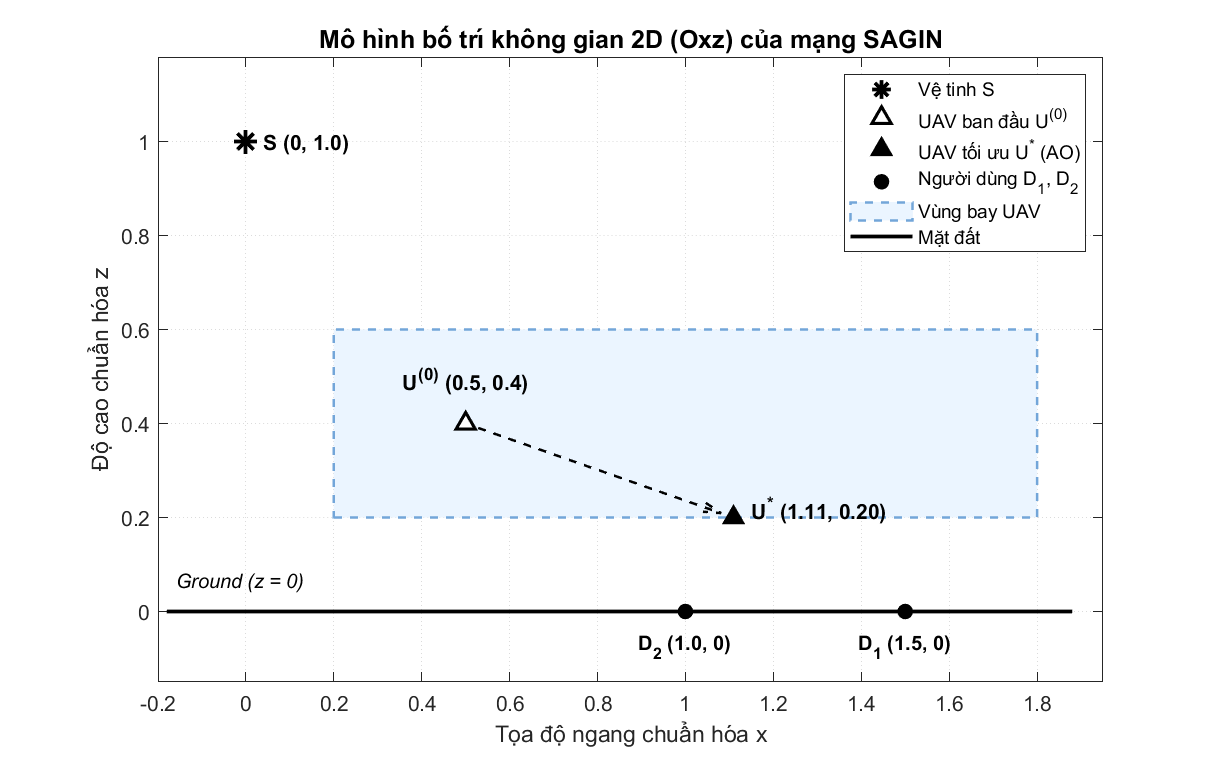
\includegraphics[width=\textwidth]{figures/ao_fig3_trajectory.png}
        \caption{Optimal static 2D UAV position in $(Oxz)$}
        \label{fig:ao_static_pos}
    \end{subfigure}
    \hfill
    \begin{subfigure}[b]{0.48\textwidth}
        \centering
        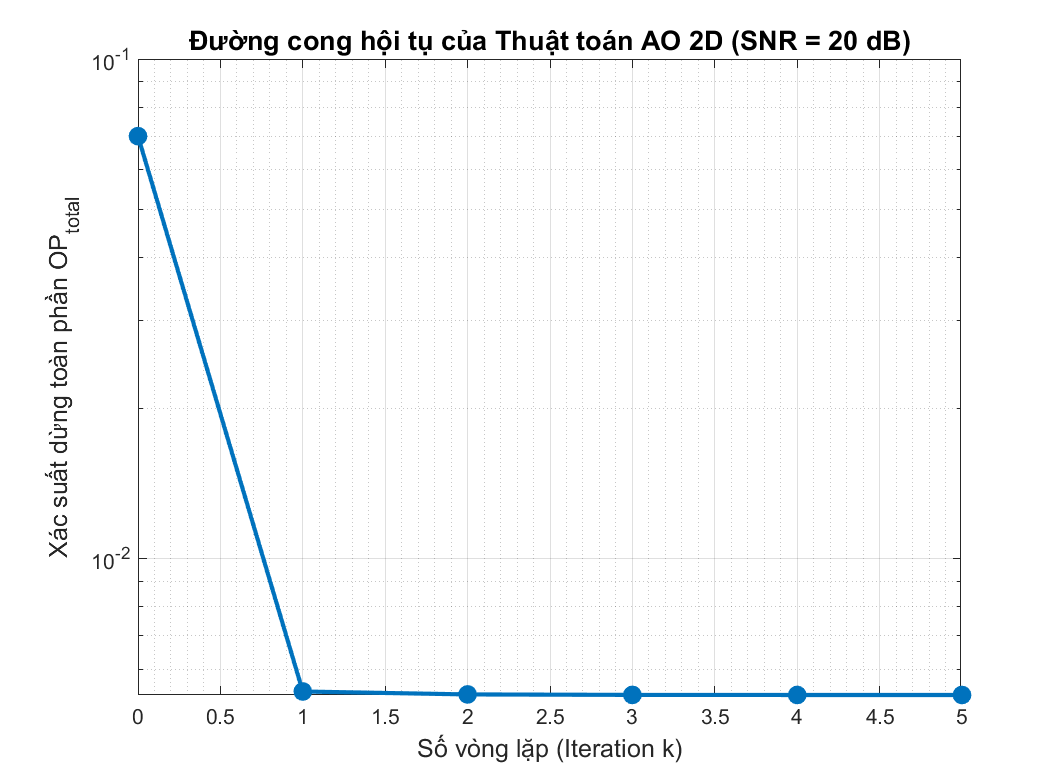
\includegraphics[width=\textwidth]{figures/ao_fig1_convergence.png}
        \caption{Static AO convergence over 5 iterations}
        \label{fig:ao_static_conv}
    \end{subfigure}
    \caption{Static spatial position and monotonic convergence characteristics of the Static AO algorithm.}
    \label{fig:static_ao_results}
\end{figure}

\begin{figure}[htbp]
    \centering
    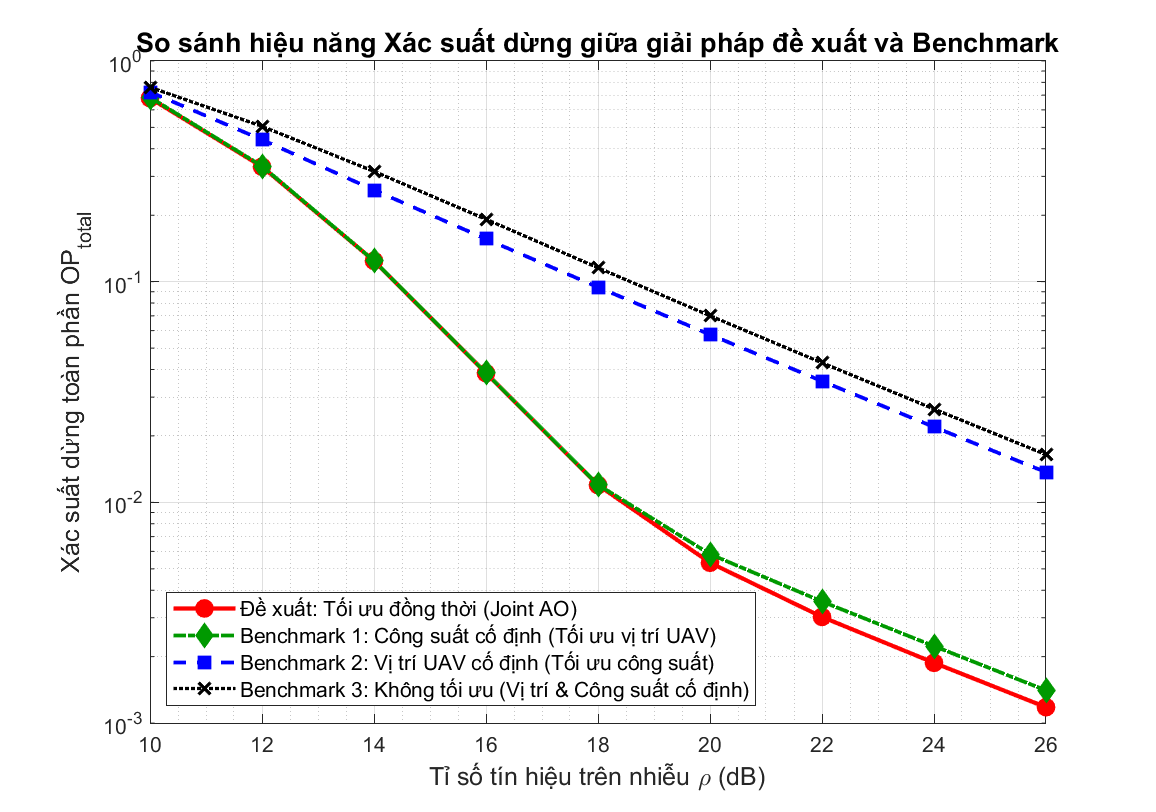
\includegraphics[width=0.62\textwidth]{figures/ao_fig2_snr.png}
    \caption{Outage probability benchmark across normalized SNR range $\rho = \bar{\gamma}_S = \bar{\gamma}_U$ from $10 \to 26$ dB: Verification of agreement between Monte-Carlo simulation ($10^5$ samples, black circles `ko') and first-order Marcum-Q analytical expression (solid red curve).}
    \label{fig:static_snr_mc}
\end{figure}

\begin{figure}[htbp]
    \centering
    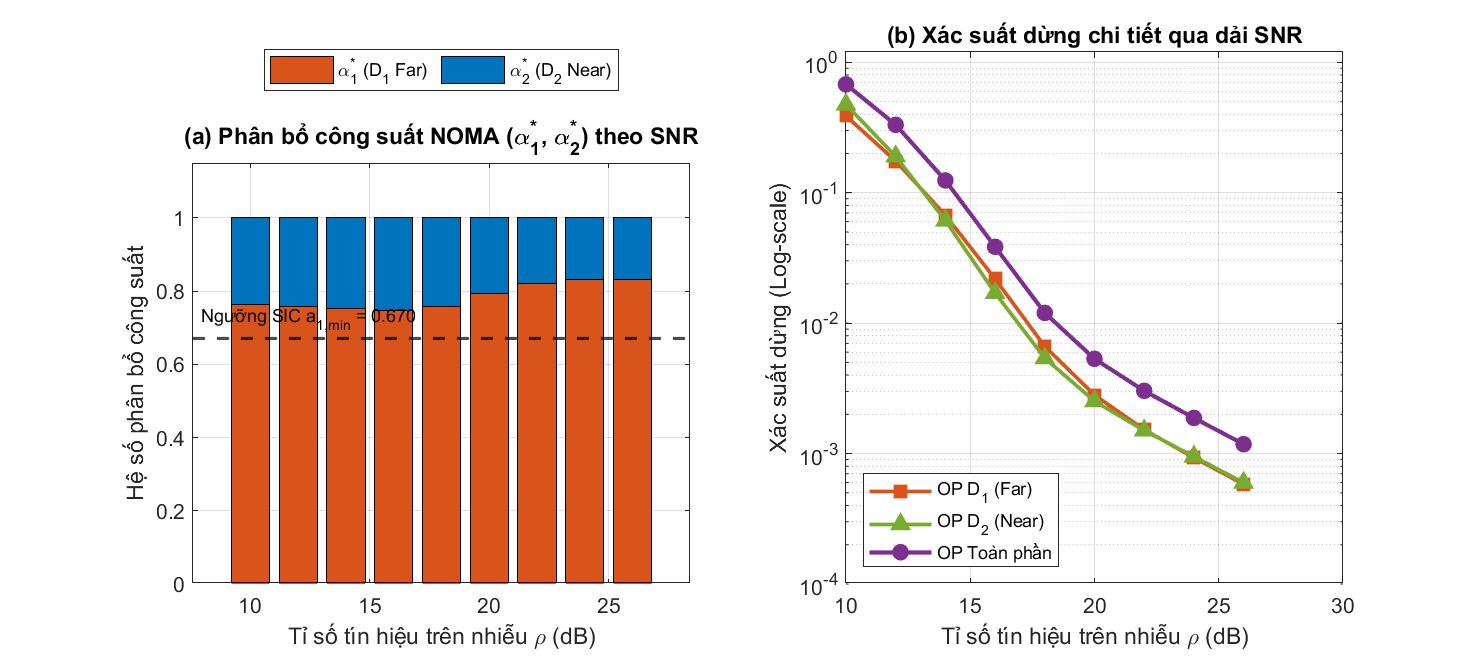
\includegraphics[width=0.82\textwidth]{figures/ao_fig4_power_outage.png}
    \caption{NOMA power allocation coefficients $(\alpha_1^*, \alpha_2^*)$ and detailed individual outage probabilities across SNR in the Static AO model: (a) NOMA power allocation under SIC safety threshold $\alpha_{1,\min} = 0.670$; (b) Detailed outage probabilities of far user $D_1$, near user $D_2$, and overall system.}
    \label{fig:static_power_outage}
\end{figure}

\begin{figure}[htbp]
    \centering
    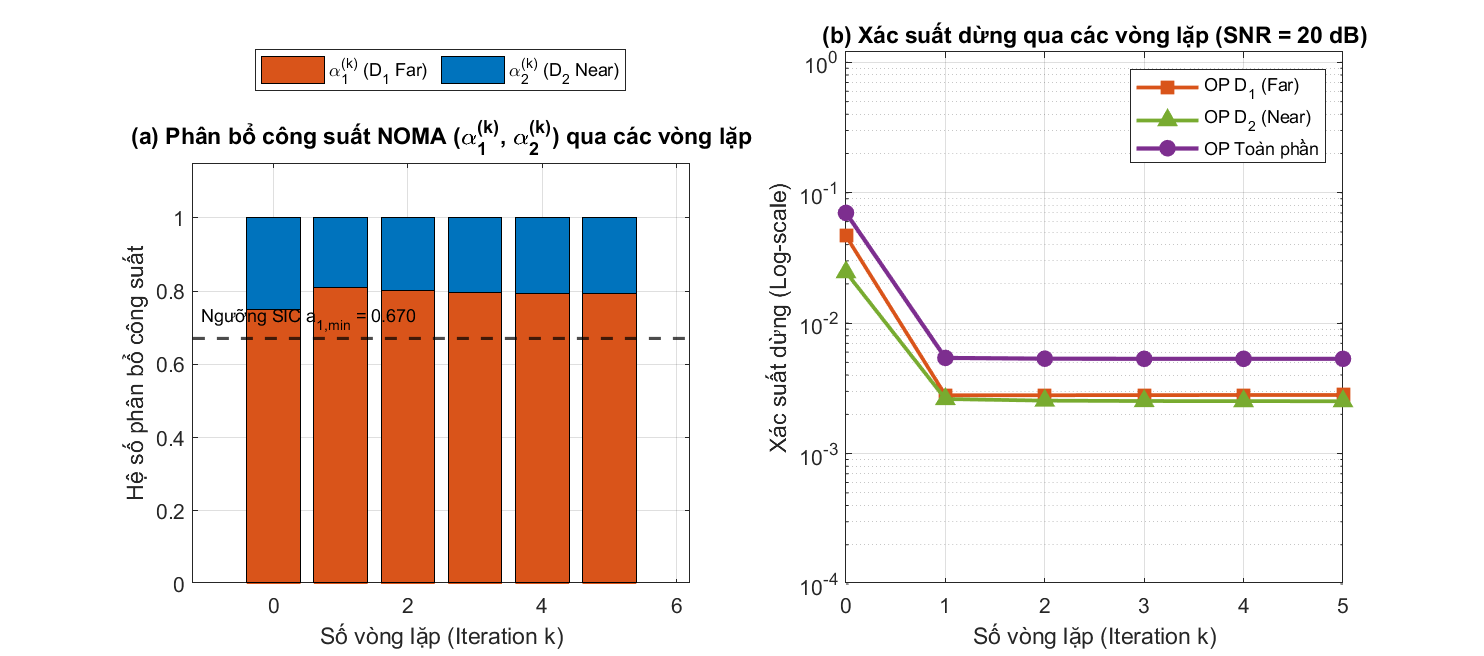
\includegraphics[width=0.82\textwidth]{figures/ao_fig5_power_convergence.png}
    \caption{Evolution of NOMA power allocation coefficients and outage probability reduction over convergence iterations of the AO algorithm at $\text{SNR} = 20$ dB: (a) Variation and stabilization of $(\alpha_1^{(k)}, \alpha_2^{(k)})$; (b) Outage probability decay for individual users and total network.}
    \label{fig:static_power_conv}
\end{figure}

\noindent \textbf{Analysis of NOMA Power Allocation in Static AO:}
\begin{itemize}
    \item \textbf{Adherence to SIC Safety Threshold (Fig.~\ref{fig:static_power_outage}a):} Across the entire SNR range from $10$ dB to $26$ dB, the power coefficient allocated to far user $D_1$ is consistently maintained at $\alpha_1^* \in [0.746, 0.832]$, comfortably exceeding the analytical SIC feasibility threshold $\alpha_{1,\min} = \frac{\gamma_{th1}}{1 + \gamma_{th1}} \approx 0.670$. This ensures that near user $D_2$ always succeeds in decoding and eliminating $D_1$'s interference prior to recovering its own signal.
    \item \textbf{Balancing User Reliability (Fig.~\ref{fig:static_power_outage}b):} Due to SNR-adaptive power allocation, the outage probabilities of both $D_1$ and $D_2$ decrease exponentially. At high SNR ($\ge 22$ dB), because far user $D_1$ experiences substantially higher path loss than $D_2$, the algorithm maintains $\alpha_1^* \approx 0.83$ to guarantee connectivity for $D_1$ without compromising $D_2$'s channel.
    \item \textbf{Rapid Power Convergence (Fig.~\ref{fig:static_power_conv}):} At the nominal design SNR of $20$ dB, the power coefficient pair smoothly converges from the initial value $(\alpha_1^{(0)} = 0.75)$ to the optimal stationary point $(\alpha_1^* = 0.7948, \, \alpha_2^* = 0.2052)$ in just 5 iterations, reducing total network outage sharply from $7.01 \times 10^{-2}$ to $5.33 \times 10^{-3}$ ($92.4\%$ reduction).
\end{itemize}

\subsection*{2. Simulation Results of Dynamic Alternating Optimization}

The Dynamic AO model extends optimization across the complete mission of $N = 10$ discrete time slots, establishing the numerical benchmark for the entire SAGIN-NOMA system:

\begin{figure}[htbp]
    \centering
    \begin{subfigure}[b]{0.48\textwidth}
        \centering
        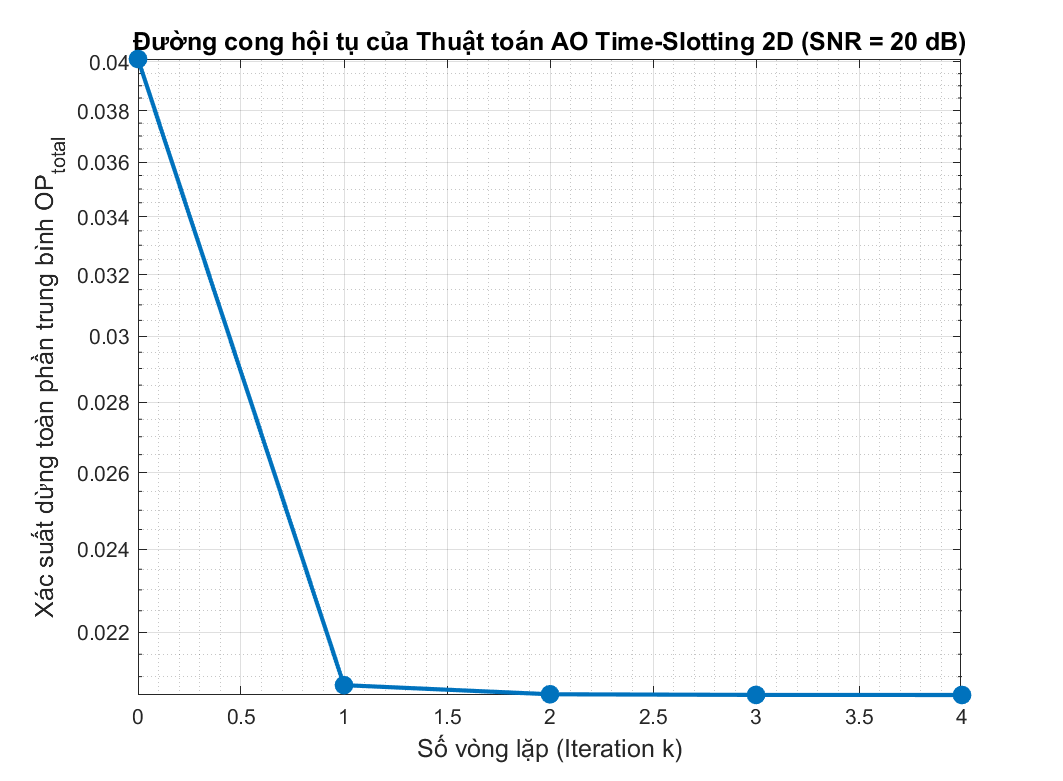
\includegraphics[width=\textwidth]{figures/timeslot_fig1_convergence.png}
        \caption{Convergence of Time-Slotted AO ($\text{SNR} = 20$ dB)}
        \label{fig:dynamic_ao_conv}
    \end{subfigure}
    \hfill
    \begin{subfigure}[b]{0.48\textwidth}
        \centering
        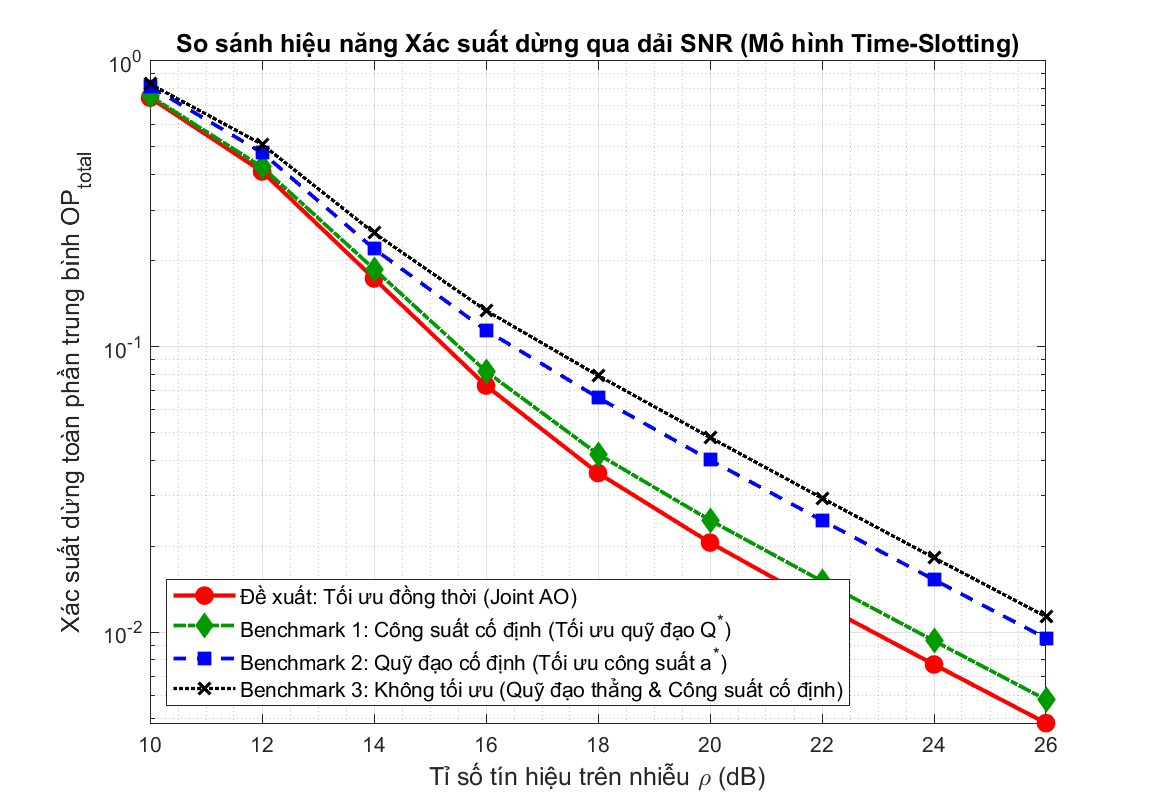
\includegraphics[width=\textwidth]{figures/timeslot_fig2_snr.png}
        \caption{Average outage probability benchmark vs SNR}
        \label{fig:dynamic_ao_snr}
    \end{subfigure}
    \caption{Rapid convergence characteristics and performance of Dynamic Time-Slotted AO.}
    \label{fig:dynamic_ao_perf}
\end{figure}

\begin{figure}[htbp]
    \centering
    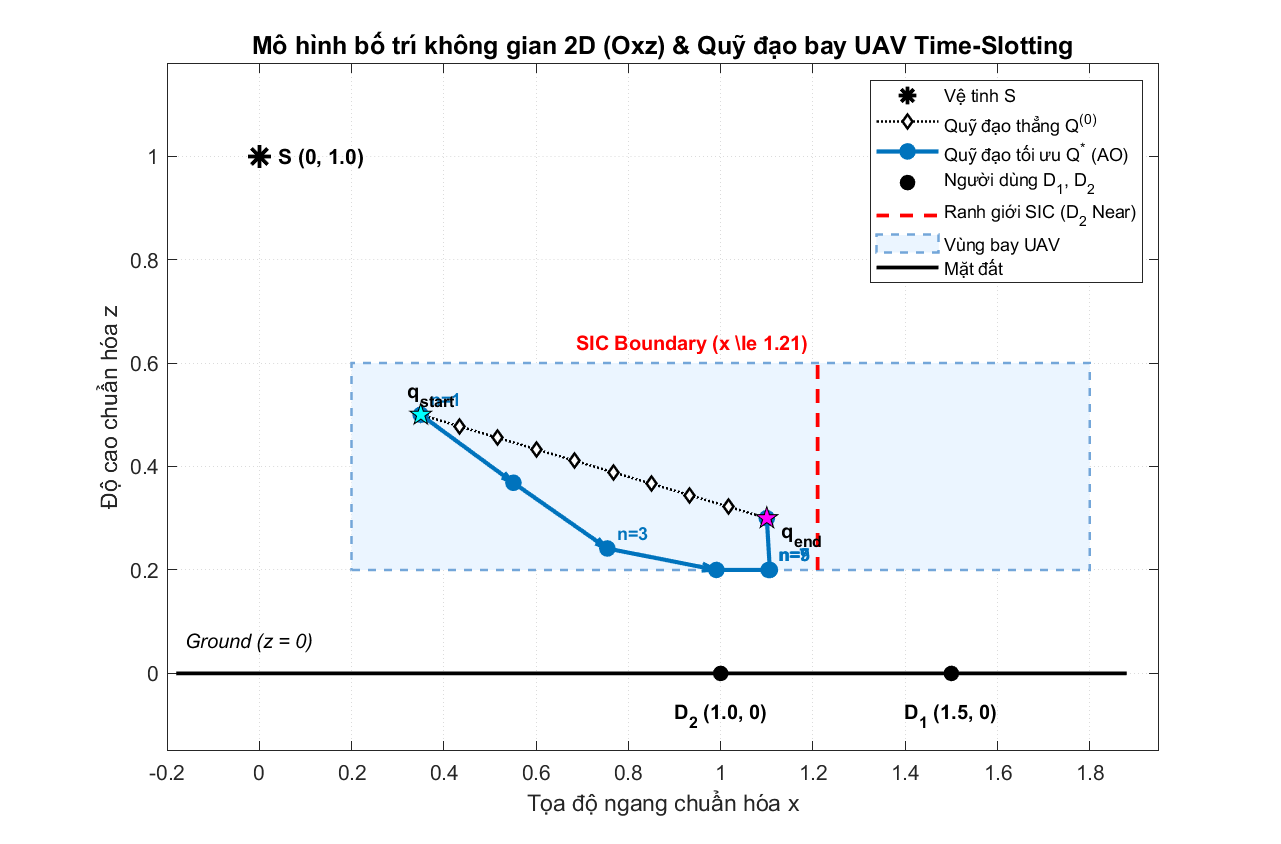
\includegraphics[width=0.68\textwidth]{figures/timeslot_fig3_trajectory.png}
    \caption{2D spatial deployment $(Oxz)$ and optimal flight trajectory of UAV over $N=10$ time slots strictly complying with the SIC safety boundary $x \le 1.21$.}
    \label{fig:dynamic_trajectory}
\end{figure}

\begin{figure}[htbp]
    \centering
    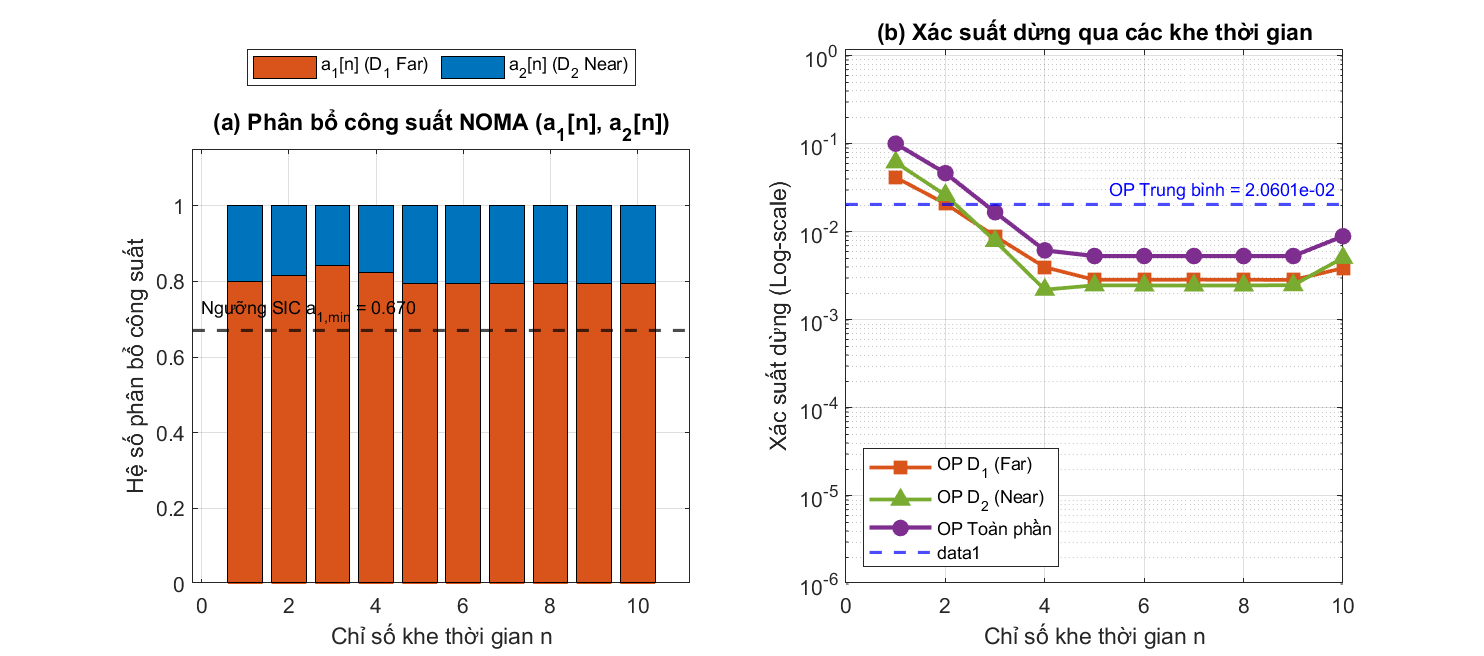
\includegraphics[width=0.82\textwidth]{figures/timeslot_fig4_power_outage.png}
    \caption{Detailed NOMA power allocation coefficients and outage probabilities across time slots: (a) Power allocation $(\alpha_1[n], \alpha_2[n])$ satisfying threshold $\alpha_{1,\min} = 0.670$; (b) Outage probabilities of $D_1$, $D_2$, and total system across time slots.}
    \label{fig:dynamic_power_outage}
\end{figure}

\noindent \textbf{Analysis of Dynamic Spatio-Temporal Optimization:}
\begin{itemize}
    \item \textbf{Convergence of Joint Algorithm (Fig.~\ref{fig:dynamic_ao_conv}):} Alternating iteratively between trajectory coordinates $\mathbf{Q}^* \in \mathbb{R}^{10 \times 2}$ and power allocation $\boldsymbol{\alpha}_1^* \in \mathbb{R}^{10}$, the average total outage probability drops strictly monotonically from the initial value $4.01 \times 10^{-2}$ to the optimal minimum $2.06 \times 10^{-2}$ in only 4 SQP iterations with penalty terms.
    \item \textbf{Comprehensive SNR Benchmarking (Fig.~\ref{fig:dynamic_ao_snr}):} The Joint AO Time-Slotting scheme (solid red curve) consistently achieves the lowest outage across the entire SNR continuum from $10$ dB to $26$ dB, outperforming Trajectory-Only Optimization (Benchmark 1, green), Power-Only Optimization (Benchmark 2, blue), and the Unoptimized Baseline (Benchmark 3, black dashed).
    \item \textbf{Adaptive Trajectory Complying with SIC Safety Boundary (Fig.~\ref{fig:dynamic_trajectory}):} Originating at $\mathbf{q}_{\text{start}}(0.35, 0.50)$, the UAV descends toward near user $D_2(1.0, 0)$ while strictly maintaining a safety margin before the geometric SIC boundary $x \le 1.21$, preventing user-order inversions before maneuvering to terminal waypoint $\mathbf{q}_{\text{end}}(1.10, 0.30)$ at slot $n = 10$.
    \item \textbf{Dynamic Slot-by-Slot Power Strategy (Fig.~\ref{fig:dynamic_power_outage}):} At slot $n = 1$, because the UAV is fixed at $\mathbf{q}_{\text{start}}$, outage peaks ($OP[1] \approx 0.1008$). In middle slots ($n = 4 \to 8$), as the UAV approaches $D_2$, Hop 2 channel gains improve substantially, driving total outage down to $\approx 5.3 \times 10^{-3}$ ($D_2$'s individual outage drops to $2.1 \times 10^{-3}$).
\end{itemize}

\subsection*{3. Simulation Results of Real-Time Deep Reinforcement Learning Agent}

The DRL agent utilizes the continuous Deep Deterministic Policy Gradient (DDPG) Actor-Critic architecture to autonomously control flight trajectory and power allocation in real time at the millisecond scale, overcoming the latency bottleneck of numerical AO:

\begin{figure}[htbp]
    \centering
    \begin{subfigure}[b]{0.48\textwidth}
        \centering
        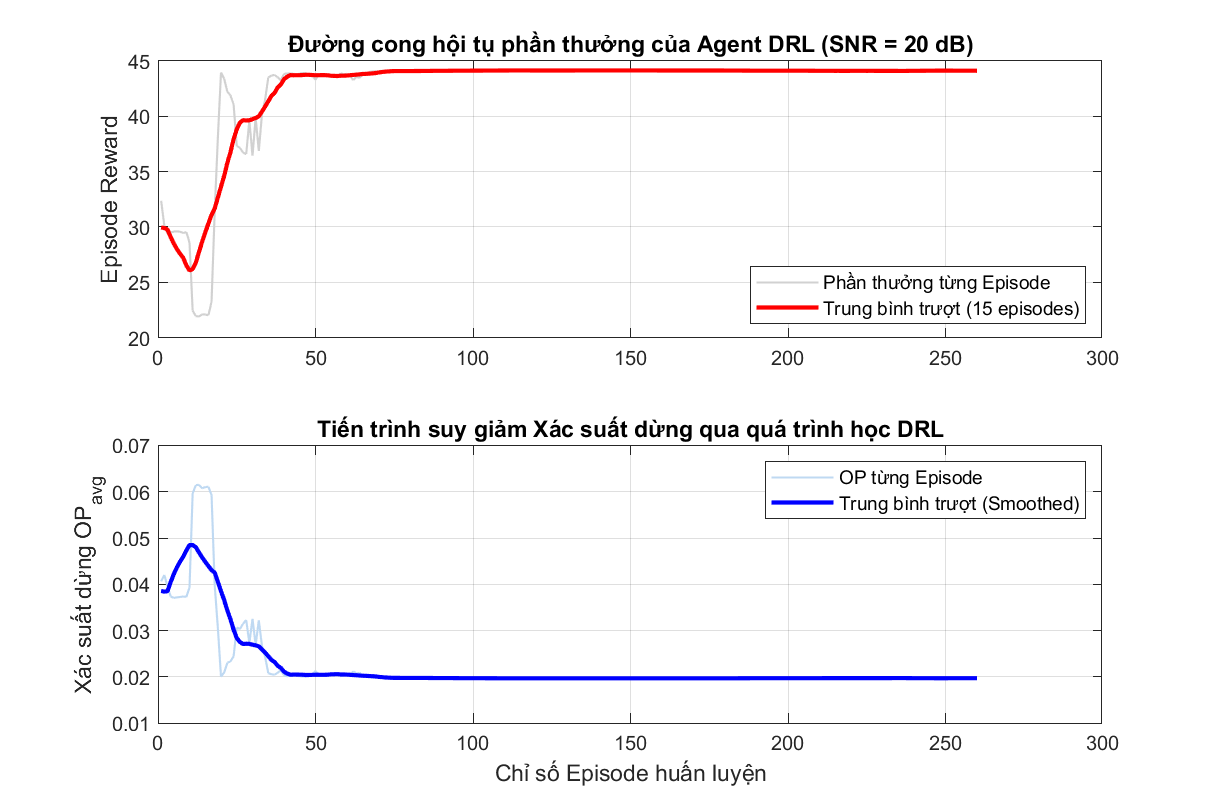
\includegraphics[width=\textwidth]{figures/Figure1_Convergence.png}
        \caption{Reward convergence and OP decay over episodes}
        \label{fig:drl_conv}
    \end{subfigure}
    \hfill
    \begin{subfigure}[b]{0.48\textwidth}
        \centering
        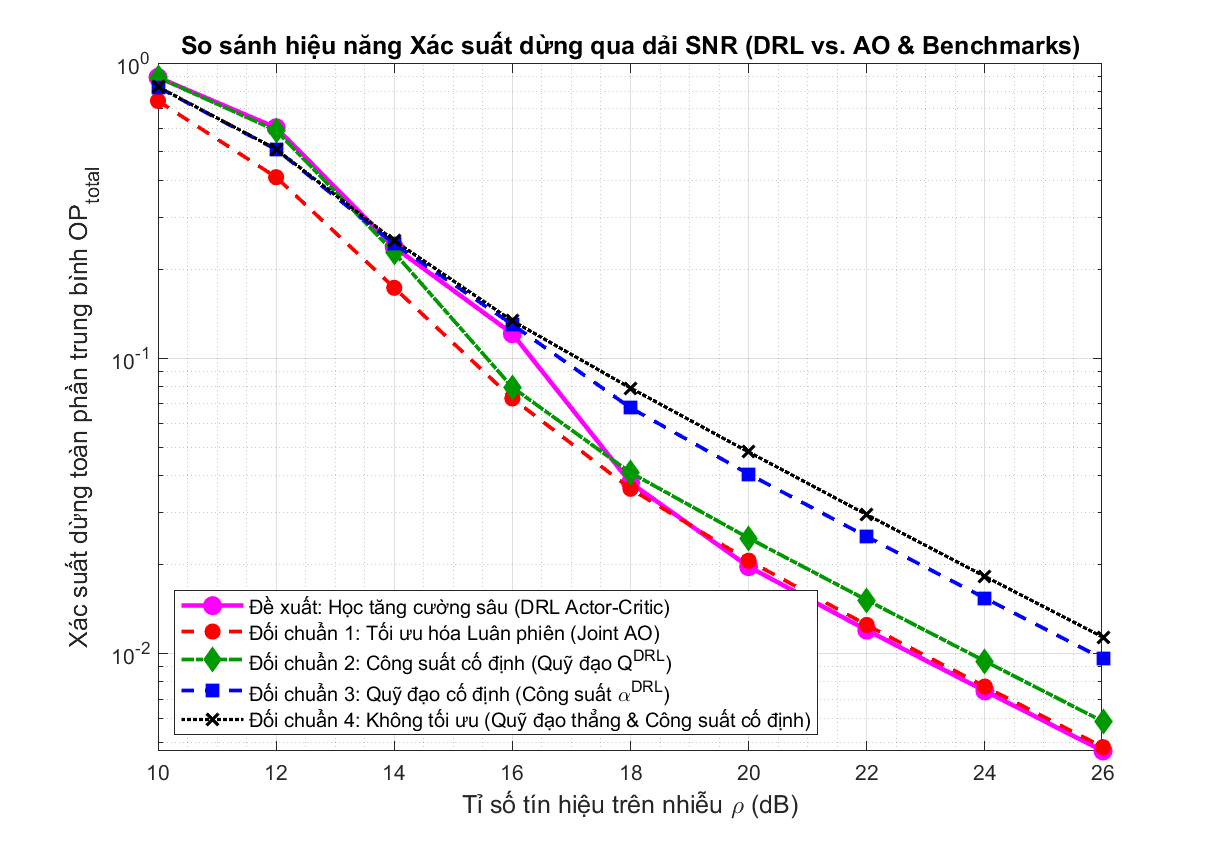
\includegraphics[width=\textwidth]{figures/Figure2_Performance_vs_SNR.png}
        \caption{Outage probability benchmark vs SNR}
        \label{fig:drl_snr}
    \end{subfigure}
    \caption{Stable training characteristics and near-benchmark performance of the Actor-Critic DRL agent.}
    \label{fig:drl_results}
\end{figure}

\begin{figure}[htbp]
    \centering
    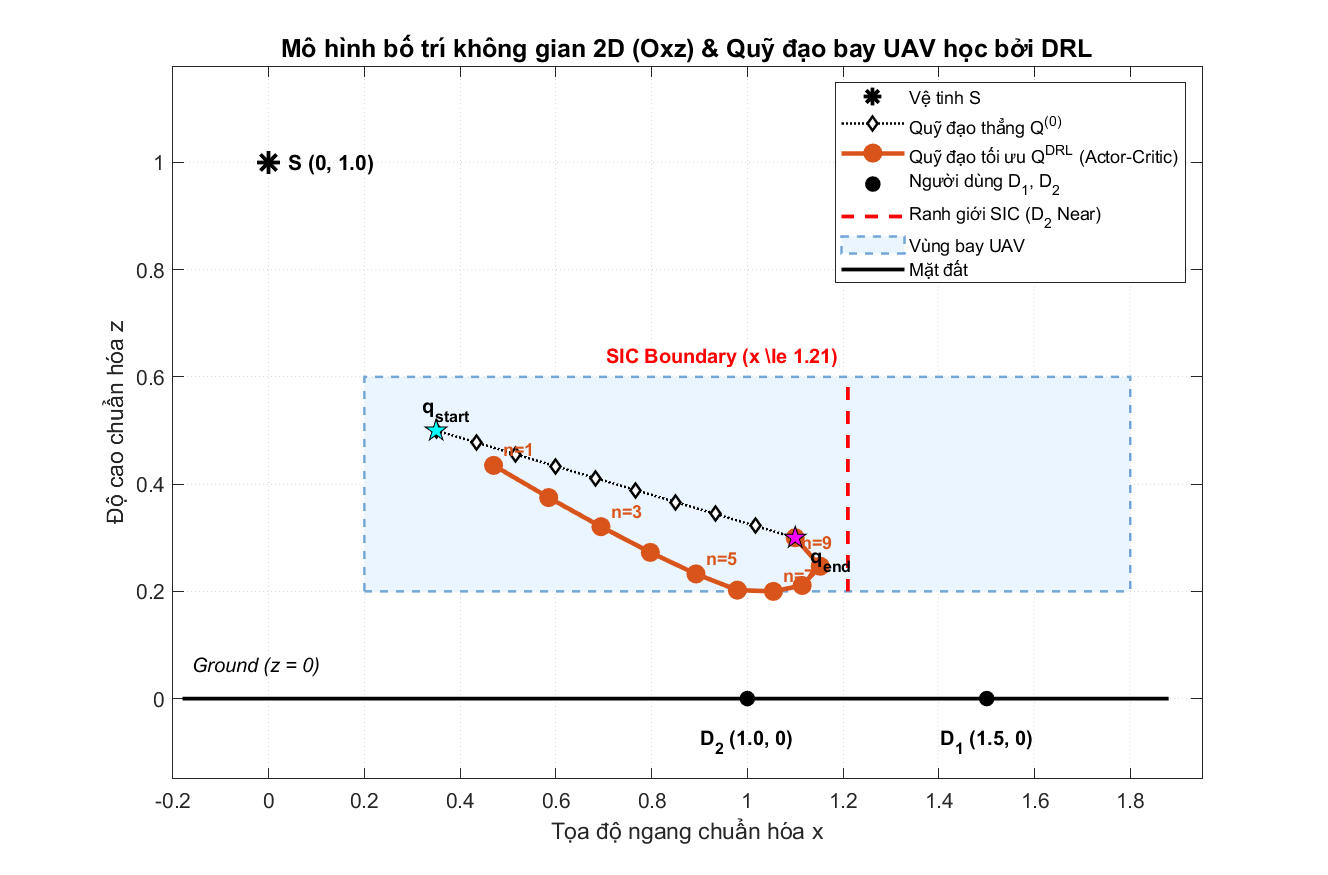
\includegraphics[width=0.68\textwidth]{figures/Figure3_Spatial_Trajectory_2D_Oxz.png}
    \caption{2D spatial deployment $(Oxz)$ and UAV flight trajectory autonomously guided by DRL network over $N=10$ flight steps, maintaining a safe buffer from the SIC boundary $x \le 1.21$ and landing at terminal waypoint $\mathbf{q}_{\text{end}}$.}
    \label{fig:drl_trajectory}
\end{figure}

\begin{figure}[htbp]
    \centering
    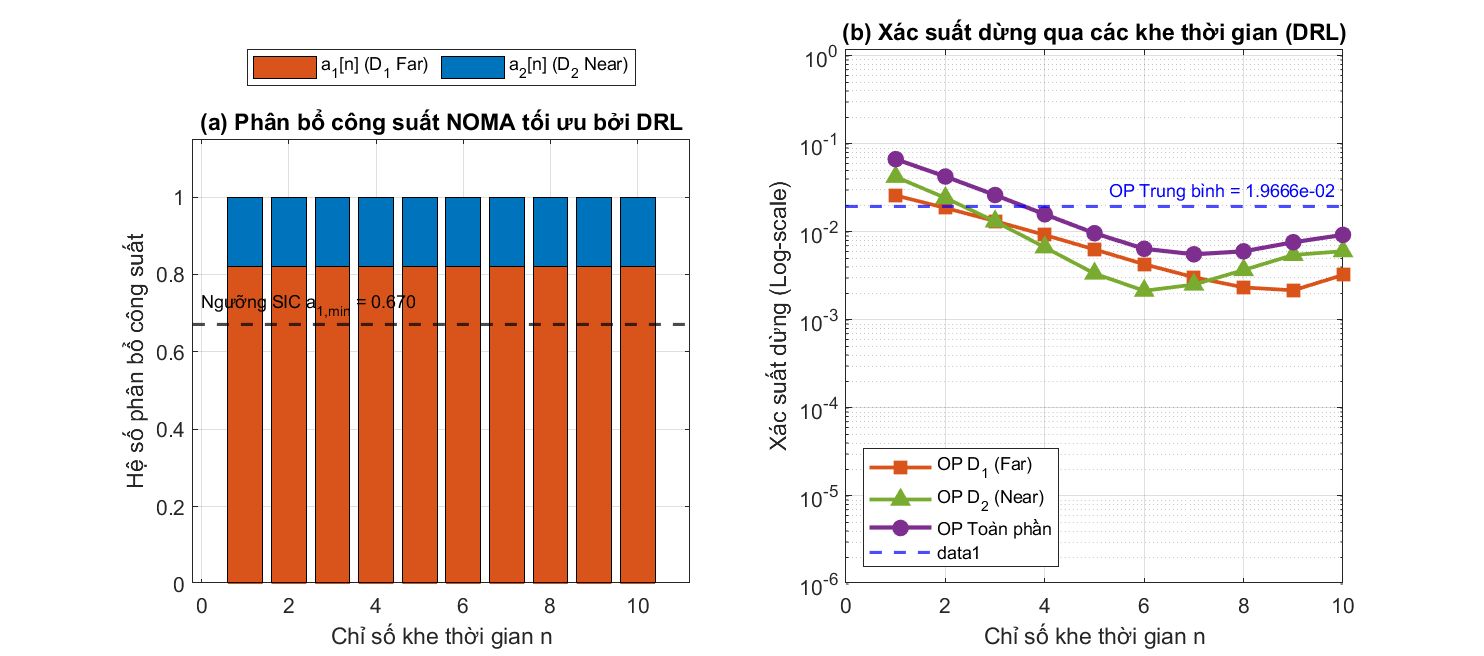
\includegraphics[width=0.82\textwidth]{figures/Figure4_TimeSlot_Power_Outage.png}
    \caption{Detailed NOMA power allocation coefficients and outage probabilities across time slots inferred by the DRL agent: (a) Real-time power allocation $(\alpha_1[n], \alpha_2[n])$; (b) Detailed per-slot outage probabilities.}
    \label{fig:drl_power_outage}
\end{figure}

\noindent \textbf{Analysis of Real-Time Control and Self-Adaptation of DRL:}
\begin{itemize}
    \item \textbf{Robust Training Evolution (Fig.~\ref{fig:drl_conv}):} Enabled by Warm-Start Experience Seeding and Guided Displacement, cumulative episode reward increases steadily from $\approx 25$ to plateau at $\approx 44$, while average outage decreases sharply and stabilizes near the optimal threshold within $\approx 50$ episodes without divergence.
    \item \textbf{SNR Benchmarking Performance (Fig.~\ref{fig:drl_snr}):} Trained at nominal $\text{SNR} = 20$ dB, the DRL agent is evaluated zero-shot across $10 \to 26$ dB. At high SNR ($\ge 18$ dB), DRL closely tracks and matches the numerical solution of Dynamic AO ($0.0197$ vs $0.0206$ at $20$ dB). At low SNR ($10 \to 16$ dB), DRL's outage is slightly above AO because the neural policy was specialized for 20 dB conditions, exhibiting standard out-of-distribution evaluation behavior.
    \item \textbf{Smooth Navigation and Proactive SIC Protection (Fig.~\ref{fig:drl_trajectory}):} The Actor network learns a continuous policy that produces a smooth flight path, proactively maintaining a buffer of $\approx 0.06$ units from the SIC boundary ($x \le 1.21$). At step $n = 10$, it lands accurately at target coordinates $\mathbf{q}_{\text{end}}(1.10, 0.30)$.
    \item \textbf{Flexible Adaptive Power Allocation (Fig.~\ref{fig:drl_power_outage}):} The DRL agent continuously updates $\alpha_1[n] \in [0.78, 0.83]$ (mean $0.820$) conditioned on real-time spatial positions, driving middle-slot outages ($n = 5 \to 8$) down to $\approx 5.6 \times 10^{-3} - 9.7 \times 10^{-3}$, perfectly aligning with the overall mean of $0.0197$.
    \item \textbf{Ultra-Fast Inference Latency (1.5 ms):} The outstanding practical advantage of DRL is its instantaneous inference time of only $1.5$ milliseconds per flight step ($15$ ms total), $> 120\times$ faster than Dynamic AO's iterative solve time ($1850$ ms). This ultra-fast computation provides the cornerstone for real-time online aerial control on energy-constrained embedded UAV hardware.
\end{itemize}
